\documentclass[a4paper]{article}
\usepackage[utf8]{inputenc}
\usepackage{fullpage}
\usepackage{csquotes}
\usepackage[ngerman]{babel}
\usepackage{float}
\usepackage{graphicx}
\usepackage{epstopdf}
\usepackage{subfigure}
\setcounter{secnumdepth}{-1} 
\usepackage{hyperref}
\usepackage{listings}
\title{Betriebssysteme Vertiefung \\ Übungskomplex 2 (Prozesse/Threads)}

\author{Dominik Eckelmann, Matr.-Nr.: 785856}
\date{\today}

\lstset{
language=C,                % the language of the code
numbers=left,                   % where to put the line-numbers
numbersep=5pt,                  % how far the line-numbers are from the code
showspaces=false,               % show spaces adding particular underscores
showstringspaces=false,         % underline spaces within strings
showtabs=false,                 % show tabs within strings adding particular underscores
frame=single,                   % adds a frame around the code
tabsize=2,                      % sets default tabsize to 2 spaces
breaklines=true,                % sets automatic line breaking
breakatwhitespace=false        % sets if automatic breaks should only happen at whitespace
}

\begin{document}

\maketitle

\tableofcontents

\section{Einleitung}
Als Teil der Lehrveranstaltung \textit{Betriebssysteme Vertiefung} im Wintersemester 2011/2012 an der \textit{Beuth Hochschule für Technik Berlin} sollte im Rahmen einer Übung mithilfe der Programmiersprache C ein Programm geschrieben werden, welches paralleles Multipliziren von Matritzen
ermöglicht.

\section{Umgebung der Tests}
Zur Zeitmessung wird ein Intel Core2Duo L7500 mit 1,6GHZ verwendet. Er verfügt über 2,9GB
adressierbaren Arbeitsspeicher. Als Betriebssystem wird Ubuntu 10.10 mit Kernel Version
2.6.35 verwendet.

Für die Tests werden zufällige Matritzen mit den größen 10, 100 und 1000 miteinander
multipliziert. Die Zeitmessung geschieht mittels der gettimeofday-Funktion.

\section{Matritzenmultiplikation}
Die Multiplikation zweier Matritzen $A$ und $B$ erfolgt über die Summenformel:
\[ c_{ij}=\sum_{k=1}^m a_{ik}\cdot b_{kj} \]
Wobei $c_{ij}$ das Element der Ergebnismatrix $C$ mit der Position $ij$.

In Listing \ref{matrix:mult} ist der C-Code zur Matritzenmultiplikation zu sehen.
Wobei a und b die beiden zu multiplizirenden Matritzen sind, result die Ergebnismatritze
und MATRIX\_SIZE die definirte größe der Matritzen.

\begin{figure}[h!]
\lstset{caption={Matritzenmultiplikation in C},
label=matrix:mult}
\begin{lstlisting}
for (i = 0; i < MATRIX_SIZE; i++) {
	for (j = 0; j < MATRIX_SIZE; j++) {
		for (k = 0; k < MATRIX_SIZE; k++) {
			if (k == 0) {
				result[i][j] = a[i][k] * b[k][j];
			} else {
				result[i][j] = result[i][j] + a[i][k] * b[k][j];
			}
		}
	}
}
\end{lstlisting}
\end{figure}

\section{Parallelisierung mit Threads}

Zum parallelisieren wird die pthread-Bibliothek verwendet.

Der verwendete Algorithmus aus Listing \ref{matrix:mult} eignet sich um
parallel verarbeitet zu werden. In dieser Arbeit wurden die Iterationen der
ersten Schleife auf die gegebene Anzahl der Threads aufgeteielt.
Hierdurch ergibt sich ein konkurierender Zugriff auf alle drei Matritzen.
Die Eingangsmatritzen a und b sind zu vernachlässigen, da auf diese lediglich
lesend Zugegriffen wird. In die Ergebnissmatrix result schreibt jeder Thread in einen
bestimmten, voneinander abgegrenzten bereich. Daher tauchen keine Seiteneffekte
durch konkurirende Zugriffe auf.

\section{Zeitmessung zu Aufgabe 1}

Die Zeitmessung ergab:
\begin{description}
\item[10x10 Matrix] 0s 162ms
\item[100x100 Matrix]  0s 8104ms
\item[1000x1000 Matrix] 8s 742103ms
\end{description}

\section{Zeitmessung zu Aufgabe 2}

Die Zeitmessung mit 2 Threads ergab:
\begin{description}
\item[10x10 Matrix] 0s 164ms
\item[100x100 Matrix]  0s 4452ms
\item[1000x1000 Matrix] 4s 950676ms
\end{description}
Es werden keine tests mit einer höheren Anzahl Threads gemacht, da das 
Testsystem lediglich 2 Threads parallel verarbeiten kann.

\section{Gegenüberstellung der Messungen}

In Abbildung \ref{graph} sind die Zeitmessungen aus Aufgabe 1 und Aufgabe 2 gegenübergestellt.
Bei der Multiplikation von 10x10 Matritzen ist noch kein unterschied der Laufzeiten zu erkennen.
Dies mag daran liegen, dass das Testsystem die gestellte Aufgabe so schnell verarbeitet, wie es
dauert einen weiteren Thread zu erzeugen.
Jedoch bei 100x100 bzw. 1000x1000 steigt der Aufwand zur Berechnung. Daher ist hier eine Verkürzung der Laufzeit mit zwei Threads gegenüber der mit einem Thread zu erkennen.

\begin{figure}
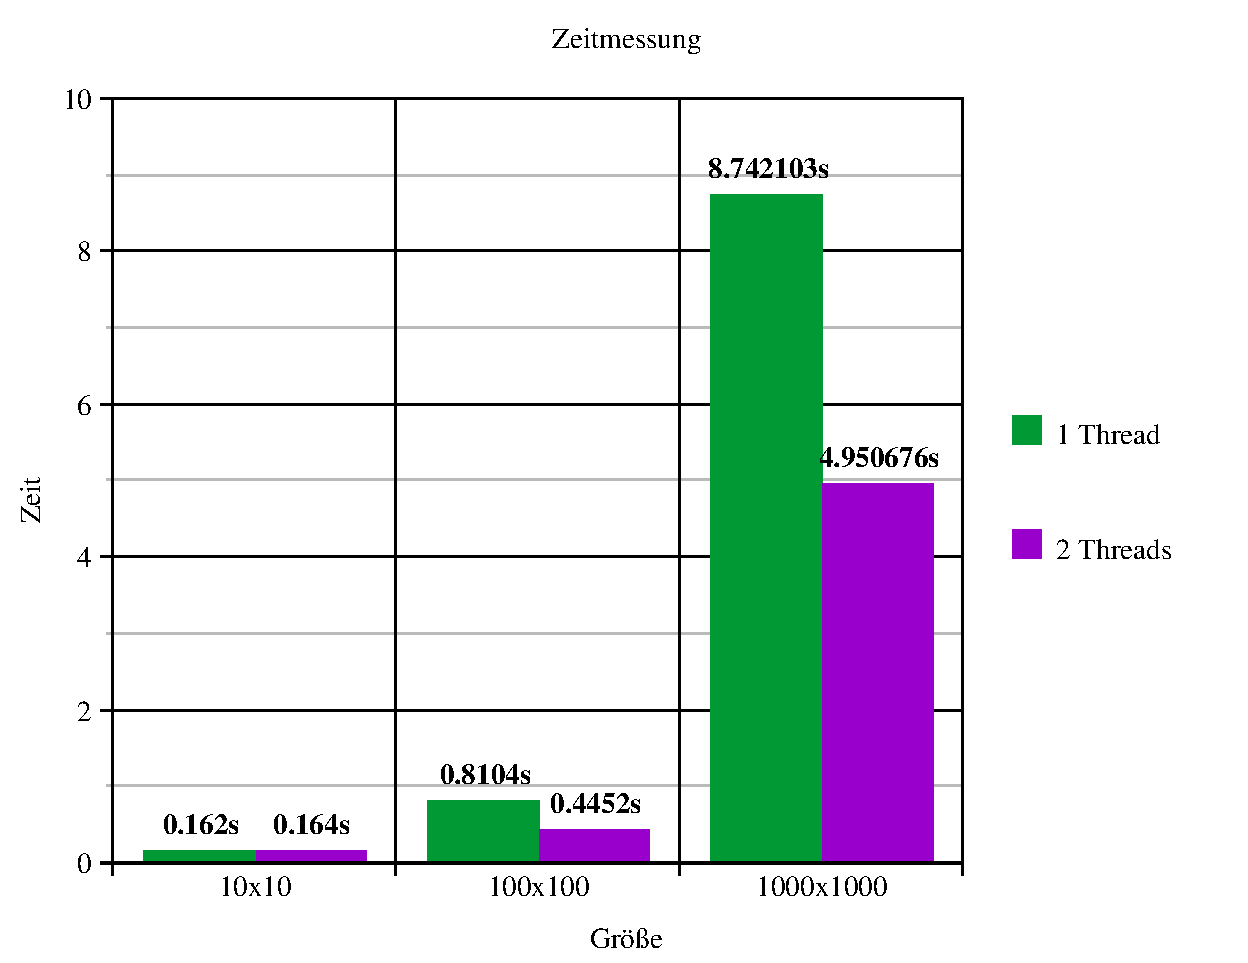
\includegraphics[scale=0.8]{graph.pdf}
\caption{Zeitmessung}
\label{graph}
\end{figure}

\end{document}